\let\negmpace\undefined
\let\negthickspace\undefined
\documentclass[journal]{IEEEtran}
\usepackage[a5paper, margin=10mm, onecolumn]{geometry}
%\usepackage{lmodern} % Ensure lmodern is loaded for pdflatex
\usepackage{tfrupee} % Include tfrupee package
\setlength{\headheight}{1cm} % Set the height of the header box
\setlength{\headsep}{0mm}     % Set the distance between the header box and the top of the text
\usepackage{gvv-book}
\usepackage{gvv}
\usepackage{cite}
\usepackage{amsmath,amssymb,amsfonts,amsthm}
\usepackage{algorithmic}
\usepackage{graphicx}
\usepackage{textcomp}
\usepackage{xcolor}
\usepackage{txfonts}
\usepackage{listings}
\usepackage{enumitem}
\usepackage{mathtools}
\usepackage{gensymb}
\usepackage{comment}
\usepackage[breaklinks=true]{hyperref}
\usepackage{tkz-euclide} 
\usepackage{listings}
% \usepackage{gvv}                                        
\def\inputGnumericTable{}                                 
\usepackage[latin1]{inputenc}                                
\usepackage{color}                                            
\usepackage{array}                                            
\usepackage{longtable}                                       
\usepackage{calc}                                             
\usepackage{multirow}                                         
\usepackage{hhline}                                           
\usepackage{ifthen}                                           
\usepackage{lscape}
\renewcommand{\thefigure}{\theenumi}
\renewcommand{\thetable}{\theenumi}
\setlength{\intextsep}{10pt} % Space between text and floats

\numberwithin{figure}{enumi}
\renewcommand{\thetable}{\theenumi}
\begin{document}
\bibliographystyle{IEEEtran}
\title{Question-1-1.11-11}
\author{EE24BTECH11035 - KOTHAPALLI AKHIL}
% \maketitle
% \newpage
% \bigskip
{\let\newpage\relax\maketitle}
\vspace{-10mm}
\textbf{Question}:\\
The scalar product of the vector $\vec{a}=\hat{i}+\hat{j}+\hat{k}$ with a unit vector along the sum of the vector $\vec{b}=2\hat{i}+4\hat{j}-5\hat{k}$ and $\vec{c}=\lambda\hat{i}+2\hat{j}+3\hat{k}$ is equal to 1. Find the  value of $\lambda$ and hence find the  unit vector along $\Vec{b}+\Vec{c}$.\\
\textbf{Solution}:\\
\begin{table}[h!]
   \centering
   \begin{tabular}{|c|c|c|}
\hline
\textbf{Line Equation} & \textbf{h value} & \textbf{m}\\
\hline
$3x - 2y + 1 = 0$ & $\left( \begin{array}{c} 3 \\ -2 \end{array} \right)$ & 1 \\
\hline
$2x + 3y - 21 = 0$ & $\left( \begin{array}{c} 2 \\ 3 \end{array} \right)$ & -21 \\
\hline
$x - 5y + 9 = 0$ & $\left( \begin{array}{c} 1 \\ -5 \end{array} \right)$ & 9 \\
\hline
\end{tabular}



   \caption{given vectors}
   \label{tabQuestion-1-1.11-11}
\end{table}   

Given vectors $\vec{a}$, $\vec{b}$, and $\vec{c}$ are:

\begin{align}
\vec{a} &= \begin{pmatrix} 1 \\ 1 \\ 1 \end{pmatrix}, \\
\vec{b} &= \begin{pmatrix} 2 \\ 4 \\ -5 \end{pmatrix}, \\
\vec{c} &= \begin{pmatrix} \lambda \\ 2 \\ 3 \end{pmatrix}
\end{align}

The sum of vectors $\vec{b}$ and $\vec{c}$ is:

\begin{align}
\vec{b} + \vec{c} &= \begin{pmatrix} 2 \\ 4 \\ -5 \end{pmatrix} + \begin{pmatrix} \lambda \\ 2 \\ 3 \end{pmatrix} \\
&= \begin{pmatrix} 2 + \lambda \\ 4 + 2 \\ -5 + 3 \end{pmatrix} \\
&= \begin{pmatrix} 2 + \lambda \\ 6 \\ -2 \end{pmatrix}
\end{align}

Now, we find the norm of $\vec{b} + \vec{c}$. The norm is given by:

\begin{align}
\|\vec{b} + \vec{c}\| &= \sqrt{(\vec{b} + \vec{c})^\top (\vec{b} + \vec{c})} \\
&= \sqrt{(2 + \lambda)^2 + 6^2 + (-2)^2} \\
&= \sqrt{(2 + \lambda)^2 + 36 + 4} \\
&= \sqrt{(2 + \lambda)^2 + 40}
\end{align}

The unit vector along $\vec{b} + \vec{c}$ is:

\begin{align}
\hat{\vec{u}} &= \frac{\vec{b} + \vec{c}}{\|\vec{b} + \vec{c}\|}
\end{align}

Given,The scalar product of $\vec{a}$ with this unit vector as 1:

\begin{align}
\vec{a}^\top \hat{\vec{u}} &= 1
\end{align}

Substituting the expressions for $\vec{a}$ and $\hat{\vec{u}}$, we get:

\begin{align}
\begin{pmatrix} 1 & 1 & 1 \end{pmatrix} \cdot \frac{1}{\sqrt{(2 + \lambda)^2 + 40}} \begin{pmatrix} 2 + \lambda \\ 6 \\ -2 \end{pmatrix} &= 1
\end{align}



\begin{align}
\frac{1}{\sqrt{(2 + \lambda)^2 + 40}} \left( (2 + \lambda) + 6 - 2 \right) &= 1 \\
\frac{1}{\sqrt{(2 + \lambda)^2 + 40}} ( \lambda + 6) &= 1
\end{align}

Squaring both sides:

\begin{align}
\frac{(\lambda + 6)^2}{(2 + \lambda)^2 + 40} &= 1
\end{align}



\begin{align}
(\lambda + 6)^2 &= (2 + \lambda)^2 + 40
\end{align}


\begin{align}
\lambda^2 + 12\lambda + 36 &= \lambda^2 + 4\lambda + 4 + 40
\end{align}

Simplifying:

\begin{align}
12\lambda + 36 &= 4\lambda + 44 \\
8\lambda &= 8 \\
\lambda &= 1
\end{align}

Thus, $\lambda = 1$. Substituting $\lambda = 1$ into $\vec{b} + \vec{c}$:

\begin{align}
\vec{b} + \vec{c} &= \begin{pmatrix} 2 + 1 \\ 6 \\ -2 \end{pmatrix} = \begin{pmatrix} 3 \\ 6 \\ -2 \end{pmatrix}
\end{align}

The norm of $\vec{b} + \vec{c}$ is:

\begin{align}
\|\vec{b} + \vec{c}\| &= \sqrt{3^2 + 6^2 + (-2)^2} = \sqrt{9 + 36 + 4} = \sqrt{49} = 7
\end{align}

Thus, the unit vector along $\vec{b} + \vec{c}$ is:

\begin{align}
\hat{\vec{u}} &= \frac{1}{7} \begin{pmatrix} 3 \\ 6 \\ -2 \end{pmatrix} = \begin{pmatrix} \frac{3}{7} \\ \frac{6}{7} \\ \frac{-2}{7} \end{pmatrix}
\end{align}

\begin{figure}[h!]
	\centering
	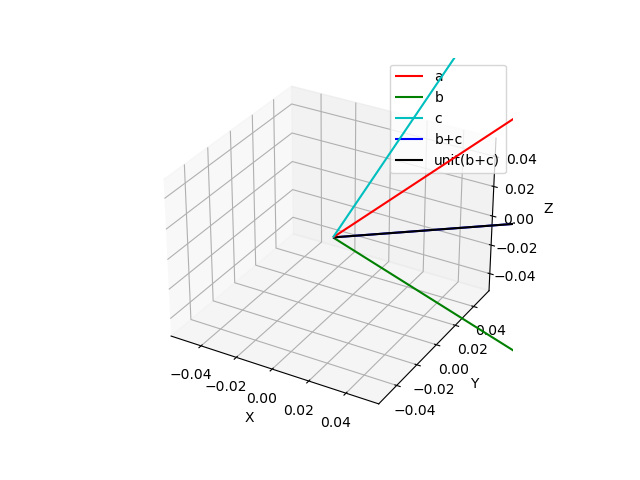
\includegraphics[width=0.5\linewidth]{figs/Figure_1.png}
	\caption{ $\vec{a},\vec{b},\vec{c}$,unit vector in the direction of  $\vec{b}+\vec{c}$}
	\label{stemplot}
\end{figure}	


\end{document}
